\documentclass[a4paper,10pt]{scrbook}
\usepackage{fontspec}
\usepackage[ngerman]{babel}
\usepackage{graphicx}
\usepackage{makeidx}
\usepackage{natbib}
\makeindex
\usepackage[colorlinks]{hyperref}
\providecommand{\tightlist}{%
\setlength{\itemsep}{0pt}\setlength{\parskip}{0pt}}
\begin{document}

another test with title z for testing sort order


 
works \includegraphics{/home/frank/Workspace8/minimalForTest/DSC08138.JPG}
but not  \includegraphics{DSC08138.JPG}
 
statt einer relativen \texttt{resources/DSC08138.JPG} referenz. Problem
in latex.

die absolute
"/home/frank/Workspace8/minimalForTest/DSC08138.JPGG"
funktioniert. der file ist
"/home/frank/Workspace8/ssg/docs/site/baked/Blog/SubBlog" in warum die
relative nicht?

An example post sorted at last and an image

\printindex
\end{document}
